\documentclass[titlepage,letterpaper,final,11pt]{scrartcl}

\usepackage[total={6.0in,8.75in},top=1.2in,left=1.35in]{geometry}

% this lets us avoid the scrartcl/hyperref conflict...
%\let\ifvtex\relax

\usepackage{verbatim}
\usepackage{empheq}
\usepackage{color}
\usepackage{animate}
\usepackage{graphicx}

% hyperref should be the last package we load
\usepackage[pdftex,
colorlinks=true,
plainpages=false, % only if colorlinks=true
linkcolor=blue,   % only if colorlinks=true
citecolor=blue,   % only if colorlinks=true
urlcolor=blue     % only if colorlinks=true
]{hyperref}

\pdfinfo{
/Title (Numerical modelling of ice sheets, streams, and shelves)
/Author (Ed Bueler)
/Subject (numerical modelling of glaciers, ice sheets, and ice shelves)
/Keywords (numerical model, numerical analysis, glacier, ice sheet, ice shelf, shallow models of ice flow)
}

\newcommand{\ddt}[1]{\ensuremath{\frac{\partial #1}{\partial t}}}
\newcommand{\ddx}[1]{\ensuremath{\frac{\partial #1}{\partial x}}}
\newcommand{\ddy}[1]{\ensuremath{\frac{\partial #1}{\partial y}}}
\newcommand{\pp}[2]{\ensuremath{\frac{\partial #1}{\partial #2}}}
\renewcommand{\t}[1]{\texttt{#1}}
\newcommand{\Matlab}{\textsc{Matlab}\xspace}
\newcommand{\bq}{\mathbf{q}}
\newcommand{\bU}{\mathbf{U}}
\newcommand{\eps}{\epsilon}
\newcommand{\grad}{\nabla}
\newcommand{\Div}{\nabla\cdot}
\newcommand{\devstress}{\tau}

\newcommand{\mname}[1]{\href{http://www.dms.uaf.edu/~bueler/mccarthy/mfiles/#1}{\texttt{#1}}}

\newcommand{\txtinput}[1]{\scriptsize\verbatiminput{#1}}

\newcommand{\txtinputtiny}[1]{\tiny\verbatiminput{#1}}

\newcommand{\mmessage}[1]{\begin{center}
\emph{see code} \url{http://www.dms.uaf.edu/~bueler/mccarthy/mfiles/#1.m}
\end{center}}

\newcommand{\mmess}[1]{\vspace{-0.1in}\begin{center}
\fbox{\url{http://www.dms.uaf.edu/~bueler/mccarthy/mfiles/#1.m}}
\end{center}}

\newcommand{\minput}[1]{\scriptsize\verbatiminput{mfiles/#1.slim.m}
\tiny\mmess{#1}\normalsize}

\newcommand{\minputtiny}[1]{\tiny\verbatiminput{mfiles/#1.slim.m}
\mmess{#1}\normalsize}

\newcommand{\alert}[1]{\emph{#1}}



\begin{document}
\graphicspath{{../photos/}{../pdffigs/}}
%\addgraphicspath{{{../pdffigs/}}


\begin{titlepage}

  \begin{center}
    {\Large\usekomafont{title} Numerical modelling of ice sheets, streams, and shelves}
    \vspace{0.5cm}

    {\large Ed Bueler}
    \vspace{1cm}

    September 2012
    %\includegraphics[width=3.3in,keepaspectratio=true]{grn-1km-csurf} \vfill
  \end{center}
\end{titlepage}


\section{preamble}

slogans:
  \begin{enumerate}
  \item \alert{focus on approximating ice flow}
  \item \alert{example numerical codes that actually work}
  \end{enumerate}
\medskip

scope:
  \begin{itemize}
  \item[$\circ$] continuum models

    \begin{itemize}
    \item shallow ice approximation (SIA) in 2D
    \item shallow shelf approximation (SSA) in 1D
    \item mass continuity \& surface kinematical equations
    \end{itemize}

  \item[$\circ$] numerical ideas

    \begin{itemize}
    \item finite difference schemes
    \item solving algebraic systems from stress balances
    \item verification
    \end{itemize}
  \end{itemize}



\emph{not} \normalsize covered here:

  \begin{itemize}
  \item Stokes and ``higher order'' flow equations
  \item thermomechanical coupling or polythermal ice
  \item subglacial hydrology/processes
  \item mass balance and snow/firn processes
  \item constitutive relations other than Glen isotropic
  \item grounding lines, calving fronts, ocean interaction
  \item paleo-climate and ``spin-up''
  \item earth deformation under ice sheet load
  \item other numerics: FEM, spectral, multigrid, parallel, \dots
  \item etc.
  \end{itemize}


\begin{center}
  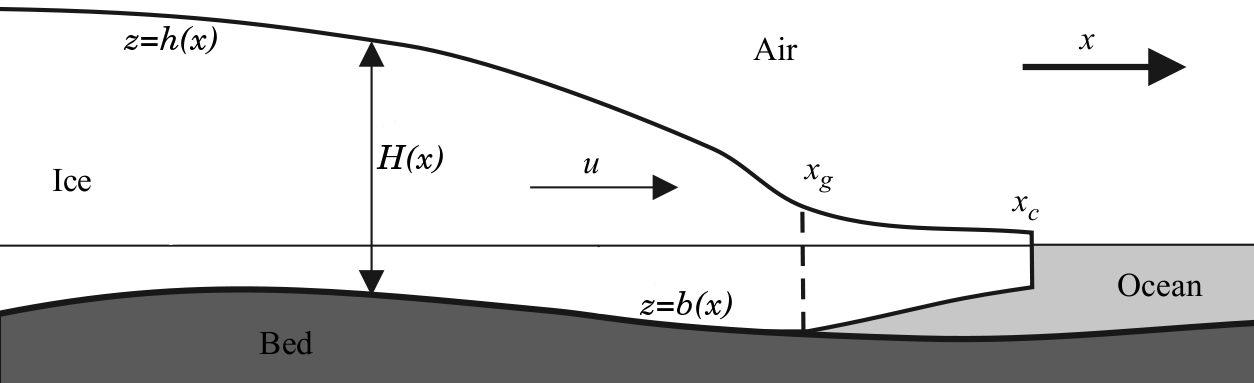
\includegraphics[width=5.0in]{flowline}

\emph{figure modified from} Schoof (2007)\nocite{SchoofMarine1}
\end{center}

  \begin{itemize}
  \item coordinates $t,x,y,z$  (with $z$ vertical, positive upward)
  \item subscripts for partial derivatives $u_x = \partial u/\partial x$
  \item $H=$ ice thickness
  \item $h=$ ice surface elevation
  \item $b=$ bedrock surface elevation
  \item $T=$ ice temperature
  \item $\mathbf{u}=(u,v,w)=$ ice velocity
  \item $\rho=$ density of ice
  \item $\rho_w=$ density of ocean water
  \item $g=$ acceleration of gravity
  \item $n=3$ Glen flow law exponent $=3$
  \item $A=A(T)=$ ice softness in Glen law ($\mathbf{D}_{ij} = A(T) \tau^{n-1} \tau_{ij}$)
  \item \alert{please ask about notation!}  (stupid questions impossible)
  \end{itemize}

%notation generally consistent with these references
\nocite{BLKCB,BBssasliding,Fowler,GreveBlatter2009,SchoofStream,SchoofMarine1}

Matlab/Octave codes:

\begin{itemize}
\item lectures are structured around 14 ice flow codes
\item each is $\sim$ 1/2 page of Matlab/Octave code
\item \texttt{.zip} and \texttt{.tar.gz} forms available from memory stick
\item online:

\centerline{\fbox{\url{http://www.dms.uaf.edu/~bueler/mccarthy/mfiles/}}}
\end{itemize}


\subsection{ice flow equations}


my first goal

\begin{itemize}
\item my goal is to get to an equation for which I can say:

\begin{center}
\emph{numerically solve just this equation, and you've got a usable model for a flowing ice sheet}
\end{center}

\item to get to my goal I will quickly recall the continuum mechanics of ice flow
\item a ``usable'' model is \emph{understood} more than it is \emph{correct}
\end{itemize}


ice in glaciers is a \emph{fluid}

\begin{itemize}
\item we describe fluids primarily by a \emph{velocity field} $\mathbf{u}(t,x,y,z)$
\item if ice fluid were
  \begin{itemize}
  \item[$\circ$] faster-moving than it actually is (e.g.: gravity stronger?), and
  \item[$\circ$] linearly-viscous like liquid water
  \end{itemize}
  
  then ice flow would be a more-familiar, ``typical'' fluid
\item in that case we would all use the Navier-Stokes equations as our flow model:
\begin{align*}
\nabla \cdot \mathbf{u} &= 0 &&\text{\emph{incompressibility}} \\
\rho \left(\mathbf{u}_t + \mathbf{u}\cdot\nabla \mathbf{u}\right) &= -\nabla p + \nu \nabla^2 \mathbf{u} + \rho \mathbf{g} &&\text{\emph{force balance}}
\end{align*}
\end{itemize}


\emph{hmmm} \dots \emph{does not sound like glaciology to me!}

is numerical ice flow modeling a part of computational fluid dynamics?

\begin{itemize}
\item \alert{yes}
\item large scale like atmosphere/ocean
\item \dots but it is a weird one
\item consider what makes atmosphere/ocean flow modeling exciting:
  \begin{itemize}
  \item[$\circ$] turbulence
  \item[$\circ$] convection
  \item[$\circ$] coriolis force
  \item[$\circ$] density/salinity variation
  \item[$\circ$] chemistry (methane, ozone, \dots)
  \end{itemize}
\item none of the above list is relevant to ice flow
\item so what could be interesting about the flow of slow, cold, stiff, laminar, inert old ice?

 \qquad \dots \qquad it's \emph{ice dynamics!}
\end{itemize}


ice is a slow, shear-thinning fluid

\begin{itemize}
\item our fluid is

  \begin{tabular}{lc}
  \emph{slow}: & $\rho \left(\mathbf{u}_t + \mathbf{u}\cdot\nabla \mathbf{u}\right) \approx 0$ \\
  \emph{non-Newtonian}: & viscosity $\nu$ is not constant
  \end{tabular}
\item ``shear-thinning'' flow: bigger strain rate means smaller viscosity
\item the standard ``full'' model is Glen-law ($n=3$) Stokes:
\begin{align*}
\nabla \cdot \mathbf{u} &= 0 &&\text{\emph{incompressibility}} \\
0 &= - \nabla p + \nabla \cdot \tau_{ij} + \rho \mathbf{g} &&\text{\emph{force balance}} \\
\mathbf{D}_{ij} &= A \tau^2 \tau_{ij} &&\text{\emph{flow law}}
\end{align*}
\item these equations above are true at every instant, and
  \begin{quote}
  \emph{geometry, boundary stress, and ice viscosity determine velocity instantaneously}
  \end{quote}
\end{itemize}


\begin{itemize}
\item ``slow'':
  $$\rho \left(\mathbf{u}_t + \mathbf{u}\cdot\nabla \mathbf{u}\right) \approx 0 \qquad \iff \qquad \begin{pmatrix} \text{forces of inertia} \\ \text{are negligible} \end{pmatrix}$$
\item a time-stepping ice sheet code recomputes the full velocity field at every time step, without requiring velocity from the previous step\footnote{to be a weatherman you've got to know which way the wind blows \dots but don't expect that from a glaciologist}
\item thus no memory of previous momentum/velocity, so
  \begin{quote}\emph{velocity is a ``diagnostic'' output of an ice flow model}\end{quote}
\end{itemize}

plane flow Stokes:

\begin{itemize}
\item in the $x,z$ plane flow case the Stokes equations say
\begin{empheq}[]{align}
u_x + w_z &= 0 &&\text{\emph{incompressibility}}\notag \\
p_x &= \tau_{11,x} + \tau_{13,z} &&\text{\emph{stress balance} ($x$)} \notag \\
p_z &= \tau_{13,x} - \tau_{11,z} - \rho g &&\text{\emph{stress balance} ($z$)} \notag \\
u_x &= A \tau^2 \tau_{11} &&\text{\emph{flow law} (diagonal)}\notag \\
u_z + w _x &= 2 A \tau^2 \tau_{13} &&\text{\emph{flow law} (off-diagonal)} \notag
\end{empheq}
\item $x,z$ subscripts are partial derivatives
\item $\tau_{13}$ is a ``vertical'' shear stress
\item $\tau_{11}$ and $\tau_{33}=-\tau_{11}$ are deviatoric longitudinal stresses 
\item we have five equations in five unknowns ($u,w,p,\tau_{11},\tau_{13}$)
\item complicated enough \dots what about in a simplified situation?
\end{itemize}


\subsection{slab-on-a-slope}

\begin{itemize}
\item rotated coordinates:
  $$\mathbf{g} = g \sin\theta\, \hat x - g \cos \theta \,\hat z$$
\item so $p_x,p_z$ equations are now:
\begin{align}
p_x &= \tau_{11,x} + \tau_{13,z} + \rho g \sin\theta \notag \\
p_z &= \tau_{13,x} - \tau_{11,z} - \rho g \cos\theta \notag
\end{align}
\end{itemize}

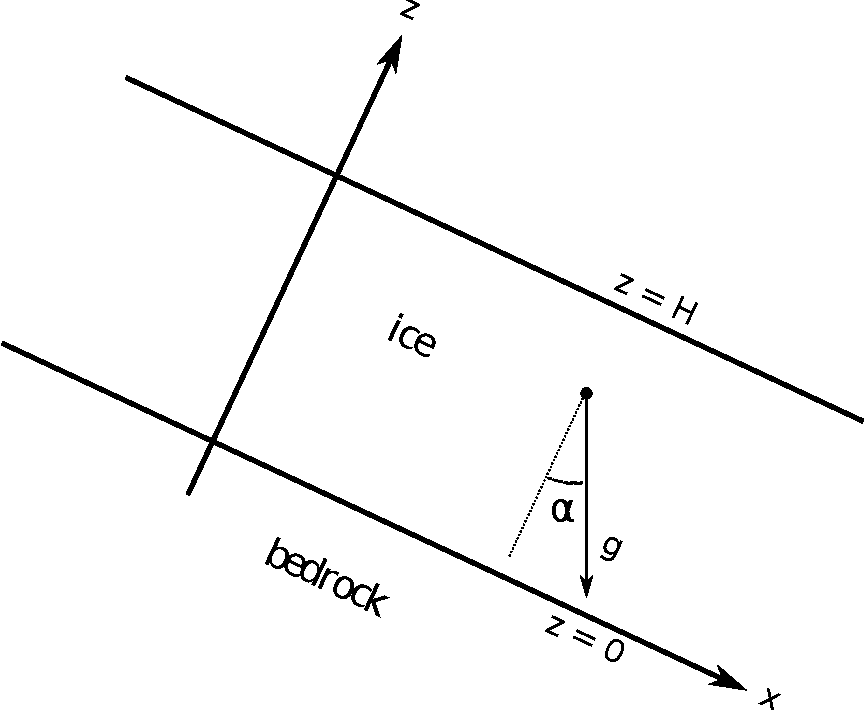
\includegraphics[width=4.0in]{slab}

\begin{itemize}
\item for a slab-on-a-slope there is \emph{no variation in} $x$
\item so equations simplify:
\begin{empheq}[box=\fbox]{align}
w_z &= 0 &   0 &= \tau_{11} \notag \\
\tau_{13,z} &= - \rho g \sin\theta &   u_z &= 2 A \tau^2 \tau_{13} \notag \\
p_z &= - \rho g \cos\theta \notag
\end{empheq}
\end{itemize}


\begin{itemize}
\item add some boundary conditions:
	$$w(\text{base})=0, \qquad p(\text{surface})=0, \qquad u(\text{base})=u_0$$
\item by integrating vertically, get :
  $$w=0, \qquad p = \rho g \cos\theta (H-z), \qquad \tau_{13} = \rho g \sin\theta (H-z)$$
\item and from ``$u_z = 2 A \tau^2 \tau_{13}$'' get
\vspace{-0.05in}
\begin{align*}
u(z) &= u_0 + 2 A (\rho g \sin\theta)^3 \int_0^z (H-z')^3\,dz' \\
     &= u_0 + \frac{1}{2} A (\rho g \sin\theta)^3  \left(H^4 - (H-z)^4\right)
\end{align*}
\end{itemize}

\begin{center}
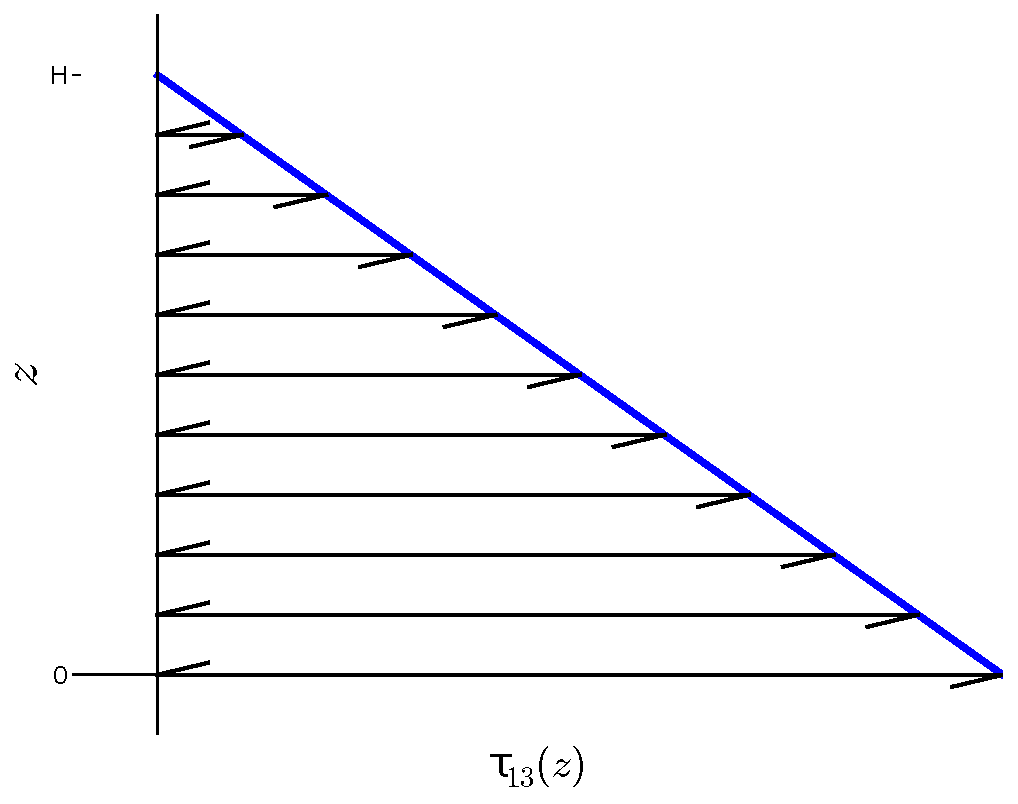
\includegraphics[width=4.0in]{slabshear}
\end{center}


\begin{itemize}
\item do we believe these equations?
\item velocity on last slide (and below) was from a \emph{formula}
\item compare to observations at right
\end{itemize}


\begin{center}
% NOT preserving aspect ratio
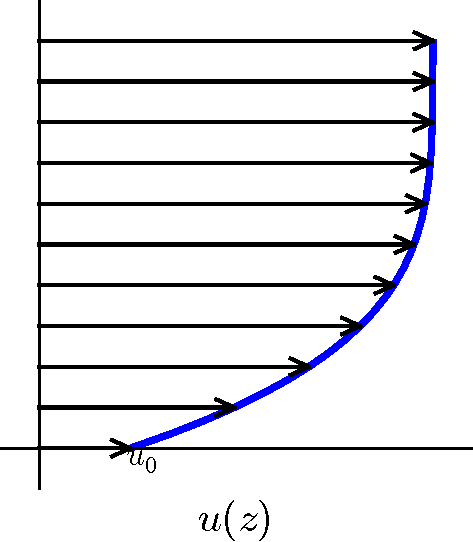
\includegraphics[width=2.5in]{slabvel} \quad 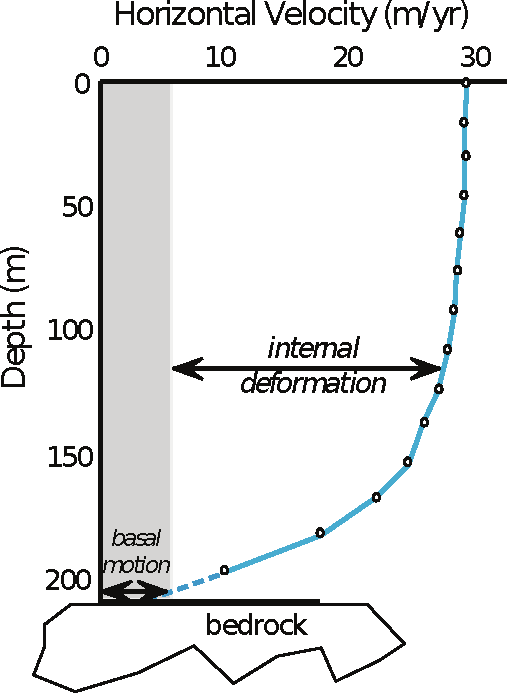
\includegraphics[width=2.5in]{athabasca_deform}
\end{center}


Velocity profile of the Athabasca Glacier, Canada, derived from inclinometry (Savage and Paterson, 1963)\nocite{SavagePaterson}


mass continuity:

\begin{itemize}
\item now we know the velocity $u=u(t,x,z)$ \dots so what?
\item suppose our slab has variable thickness $H(t,x)$
\item compute the vertical average of velocity:
	$$\bar u(x,t) = \frac{1}{H}\int_0^{H} u(t,x,z)\,dz$$
\end{itemize}

\begin{itemize}
\item consider change of area (ice volume in 3D) in the figure:
	$$\frac{dA}{dt} = \int_{x_1}^{x_2} M(x)\,dx + \bar u_1 H_1 - \bar u_2 H_2$$
\item but, assuming width $dx=x_2-x_2$ is small, $A\approx dx\, H$; divide by $dx$ and get
   $$H_t = M - \left(\bar u H\right)_x$$
\item this is a \emph{mass continuity equation}
\item I'll return to this topic \dots
\end{itemize}

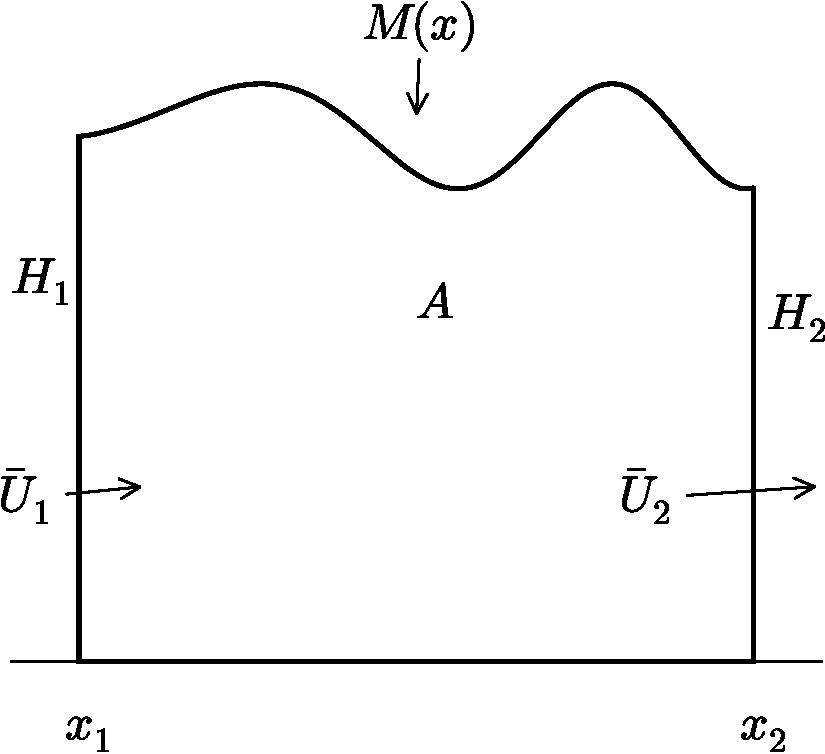
\includegraphics[width=3.0in]{slabmasscontfig}


rough explanation of ``shallow ice approximation'' (SIA)

\begin{itemize}
\item from slab-on-slope velocity formula in $u_0=0$ case (``non-sliding SIA''),
\begin{align*}
\bar u H &= \int_0^H \frac{1}{2} A (\rho g \sin\theta)^3  \left(H^4 - (H-z)^4\right)\,dz \\
	&= \frac{1}{2} A (\rho g \sin\theta)^3  \left(\frac{4}{5} H^5\right) \\
	&= \frac{2}{5} A (\rho g \sin\theta)^3 H^5
\end{align*}
\item note $\sin \theta \approx \tan\theta = - h_x$
\item combine with mass continuity $H_t = M - \left(\bar u H\right)_x$:
  $$H_t = M + \left(\frac{2}{5} (\rho g)^5 A H^5 |h_x|^2 h_x\right)_x.$$
\item I'll return to this topic \dots
\end{itemize}



%         References
\clearpage\newpage
\bibliography{ice_bib}
\bibliographystyle{siam}

\end{document}